\chapter{Details of the Heusler dynamics and corresponding DFT calculations}	

\section{Further details of the experimental setup}

Figure \ref{fig: Heuslerstatic} plots the experimentally measured static asymmetry for the A2 and B2 phases. Note that in the B2 phase, the magnetic signal from Co is smaller than the asymmetry signal in the A2 phase, while the Mn signal is larger in the B2 phase than the A2 phase. In Fig. S2B, we show that the predicted magnetic moment per atom agrees with experimental measurements for both the Mn and Co magnetic asymmetry signal, which validates the use of our DFT calculations to explain the dynamical measurements (see also section 6 of this Appendix).

\begin{figure}[htbp]
	\begin{center}
		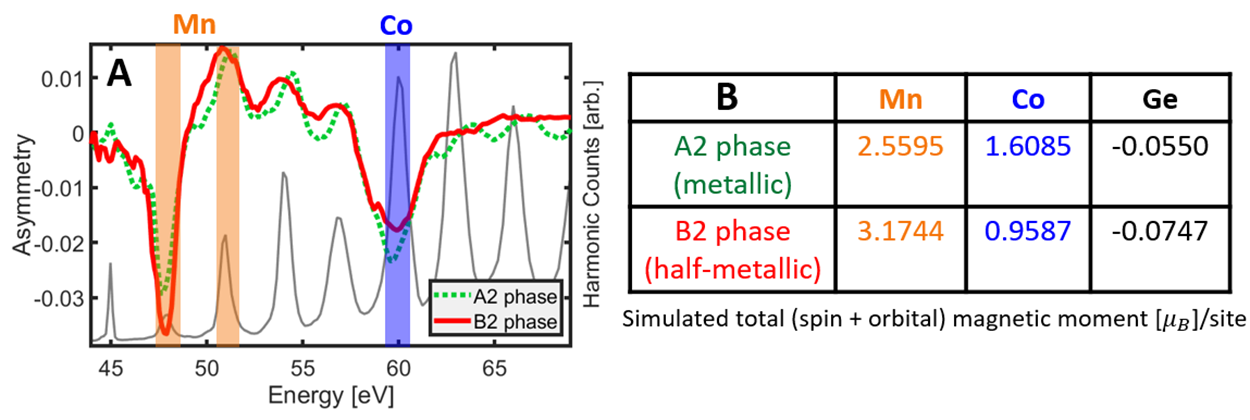
\includegraphics[width=150mm]{figs/Heuslerstatic}
	\end{center}
	\caption{(A) Static asymmetry measurements for the two phases of the material. The magnitude of the magnetic signal in Co is larger in the A2 phase, while that of Mn is larger in the B2 phase. (B) DFT calculation of the magnetic moment for each element in compound. The increase in magnetic moment for Co and decrease in the magnetic moment for Mn in the A2 phase (compared to the B2 phase) is consistent with these values.}
	\label{fig: Heuslerstatic}
\end{figure}

\section{Sample preparation}

Samples were dc magnetron sputter deposited at room temperature with the following thin film structure: SiO$_2$ / 5 nm Ta / 10 nm Co$_2$MnGe (CMG) / 2.8nm Ta. The CMG layer was formed by co-sputtering from a Co$_2$Mn target and the pure Ge target. The CMG is quasi-amorphous in the as-deposited state as confirmed by x-ray diffraction.  The samples are ex situ annealed in high vacuum at or above 240 °C to form a crystalline structure. Below 240 °C, the structure remains quasi-amorphous with high resistivity and low magnetic moment. We previously showed in Ref. \cite{Shaw2018} that the A2 structure, which is metallic, dominates at annealing temperatures at or below 280 C. However, above 300 C, the structure is B2 with a half metallic bandstructure.  Both the crystalline structure and half-metallic electronic structures were verified through x-ray diffraction, magnetometry and ferromagnetic resonance spectroscopy \cite{Shaw2018}.

\section{Change in reflectivity due to optical excitation in both phases} 
To further verify that the transient enhancement observed in Fig. 2A of the main text does not arise from any optical artifacts such as a change in the refractive index due to electronic contributions, we measured the change in the reflectivity of the sample with s-polarized light at the Co M-edge and compared this signal in the B2 phase (where the transient enhancement occurs), to the A2 phase (which has identical chemical composition but no transient enhancement). When measuring in our geometry (as shown in Fig. S1) with s-polarization, there are no magnetic contributions to the change in reflectivity. This transient reflectivity is plotted in Fig. \ref{fig: ReflectivityHeusle}. Note that the magnitude of the signals (to within error) are identical. This confirms that the findings in the main text arise from changes in the magnetic moment of Co in the B2 phase.

\begin{figure}[htbp]
	\begin{center}
		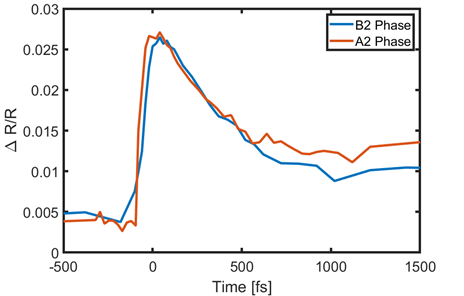
\includegraphics[width=150mm]{figs/ReflectivityHeusler}
	\end{center}
	\caption{Change in reflectivity measured for both the A2 and B2 phases. Note that to within experimental error, the signal is identical for the two samples. This confirms that the non-magnetic contribution to the signal is the same, while the magnetic signal is the cause of the transient enhancement.}
	\label{fig: ReflectivityHeusler}
\end{figure}

\section{Element averaged response of the A2 and B2 phases}
Given that the element resolved MOKE signal has all information on the total magnetization of the sample (to within 3 orders of magnitude), we can use it to construct the element averaged signal (that would be measured by an element averaging probe such as visible MOKE). This signal is plotted in Fig. \ref{fig: ElementAveMOKE} along with the element specific response. Note that for the element averaged signal, no transient enhancement would be detected.

\begin{figure}[htbp]
	\begin{center}
		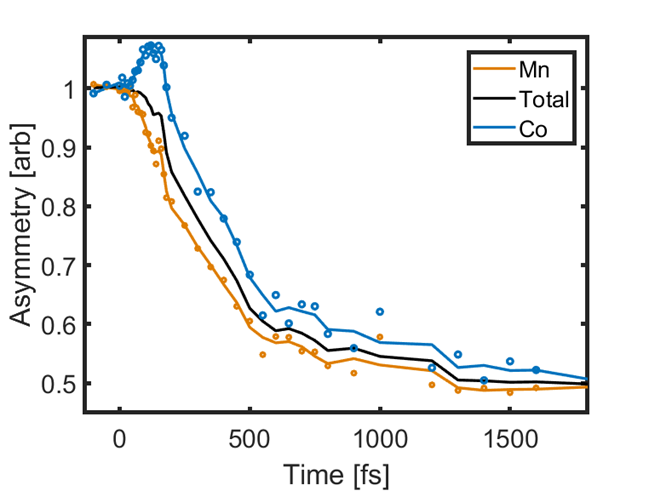
\includegraphics[width=120mm]{figs/ElementAveMOKE}
	\end{center}
	\caption{Total magnetization of sample plotted with element resolved signal. Total signal constructed from the weighted contributions of the Mn and Co magnetizations measured with TMOKE.}
	\label{fig: ElementAveMOKE}
\end{figure}

\section{Dynamics of Co$_2$MnGe on $\alpha$-Al$_2$O$_3$}

To confirm that the transient enhancement of Co in Co$_2$MnGe in the B2 phase is ubiquitous for the material, and not influenced by the choice of substrate, we grew samples of CMG on sapphire rather than SiO$_2$. The composition was: 2.8 nm Ta / 10 nm CMG / 5 nm Ta / $\alpha$-Al$_2$O$_3$. The results are shown in Fig. \ref{SapphireHeusler}. Due to a more transparent stack with less total fluence absorbed by the CMG, both the quenching and magnitude of the transient enhancement observed was significantly smaller than observed on the sample deposited on SiO$_2$. Note that the enhancement is still very clearly noticeable.

\begin{figure}[htbp]
	\begin{center}
		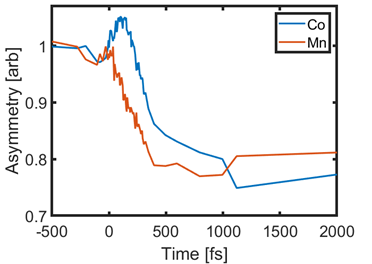
\includegraphics[width=120mm]{figs/SapphireHeusler}
	\end{center}
	\caption{Element resolved dynamics of Co2MnGe (B2 phase) on sapphire.}
	\label{fig: SapphireHeusler}
\end{figure}

\section{Method for calculating density of states and magnetic moments from density functional theory}
The density of states and magnetic moments of B2 and A2 phases of Co$_2$MnGe has been calculated by means of density functional theory \cite{Hohenberg1964,KOHN1965}  as implemented in the spin-polarized relativistic Korringa-Kohn-Rostoker (SPR-KKR) code \cite{Kruglyak2010}. The chemical disorder were treated within the coherent potential approximation (CPA) \cite{Ebert2011,Soven1967} We used the Vosko-Wilk-Nusair \cite{Stocks1978} version of the local spin density approximation for the exchange-correlation functional. The shape of the potential was considered by using both the atomic sphere approximation (ASA) solving the full relativistic Dirac equation (to obtain orbital and spin magnetic moments) and the full potential (FP) scheme combined with scalar relativistic approximation (to calculate DOS). We sample the irreducible wedge of the Brillouin zone with 1500 k-points for the magnetic moment calculations and 16000 for the density of states (DOS) calculations. For all simulations the $s$, $p$, $d$, $f$ orbitals have been included in the basis set ($l_{max}$ = 4). All parameters were calculated for a cubic Heusler structure at the experimental lattice parameter of Co$_2$MnGe 5.814 $A$. Neither the tetragonal distortion and change in lattice parameter nor the 2 percent Ge excess has significant effect on the estimated parameters.

\section{Probabilities for laser-driven transitions in the B2 and A2 phases}

To gain insight into the laser-induced electronic excitations, we calculated the transition probabilities, shown in Fig. \ref{fig: Heus4}. These results were obtained from the DOS curves obtained for the B2 and A2 phases, shown in Fig. \ref{fig: Heus3}. This information was deduced by employing the Fermi's Golden rule within the dipole approximation:
\begin{equation}
I(\omega)=\frac{2\pi}{\hbar}\sum_{k,i,f}\braket{\Psi_{f,k}|del|\Psi_{i,k}}\delta(E_{f,k}-E_{f,k}-\omega)
\label{eqn:HeuslerS1}
\end{equation}
where $I(\omega)$ stands for the absorption intensity of the incident light with energy $\omega$ and $\ket{\Psi_{i,k}}$ ($\ket{\Psi_{f,k}}$) are the occupied (unoccupied) Bloch states, characterized by wavevector $k$ and the corresponding eigenenergy $E_{i,k}(E_{f,k})$.

By projecting the Bloch states onto the atomic site a and angular momentum $l$ and spin $\sigma$ ($\ket{a,l,σ}$), one can decompose the intensity given by Eq. \ref{eqn:HeuslerS1} into the atom-resolved contributions:
\begin{equation}
I(\omega) \approx \frac{2\pi}{h}\sum_{\alpha,l,\sigma}\sum_{\alpha',l',\sigma'}\sum_k\braket{\Psi_{f,k}|a,l,\sigma}\braket{a,l,\sigma|del|a',l',\sigma'}\braket{a',l',\sigma'|\Psi_{i,k}}\delta(E_{f,k}-E_{i,k}-\omega)
\end{equation}
Furthermore, we can neglect the spin-flip transitions due to the smallness of spin-orbit coupling and take advantage of the fact that the matrix elements of the gradient operator for Co and Mn states are similar to each other (Mn 3$d$-4$p$ transition matrix elements are 6 percent larger than that for Co). Then we end up with the following expression:
\begin{equation}
I(\omega) \approx \frac{2\pi}{h}\sum_{\alpha,l,l',\sigma}\sum_k\int^{E_F}_{-\inf}d\omega'N_{\alpha,l',\omega,k}^{occ}\dot N^{unocc}_{\alpha,l',\sigma,k}(\omega' + \omega)\delta_{l-l'-1}
\label{eqn:HeuslerS4}
\end{equation}
The DOS of occupied states is multiplied with a Fermi-Dirac distribution $f_{F-D}(\omega)$ at room temperature and that of unoccupied with (1-$f_{F-D}(\omega)$.

As one can see, the DOSs for the same $k$ enter the summation, meaning that only $k$-conserving transitions are taking place, as usual for optical excitations. We have also verified that averaging the $k$-resolved DOS before summing them up marginally changes the results. This will be shown in Section B8 below. Thus, we employed a further simplified formula for the analysis of experimental data:

\begin{equation}
I(\omega)\approx\frac{2\pi}{h}\sum_{\alpha,l,l',\sigma}\int^{E_F}_{-\inf}d\omega'N^{occ}_{a,l,\sigma}(\omega')\dot N^{unocc}_{a,l',\sigma}(\omega'+\omega)\delta_{l-l'-1}
\label{eqn:HeuslerS5}
\end{equation}
An analysis based on such a simple expression allows for a straightforward interpretation of the experimental data at least on a qualitative level. Most importantly, it correctly captures the differences in the behavior of Co and Mn magnetic moments after the laser irradiation.

We have found that the main contribution comes from the transitions between $d$ and $p$ states ($s$-$p$ and $d$-$f$  transitions are less intense). Thus, to calculate the transition probabilities, we used the projected DOS for the B2 and A2 phases, shown in Fig. \ref{fig: elementOrbitalDOS}.

\begin{figure}[htbp]
	\begin{center}
		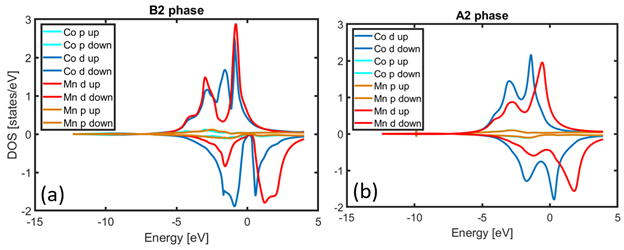
\includegraphics[width=150mm]{figs/ElementOrbitalDOS}
	\end{center}
	\caption{Element and orbital specific DOS for (a) B2 and (b) A2 phases. Note that the p orbitals are an order of magnitude smaller than the d orbitals, however transitions take place from p to d or d to p orbitals.}
	\label{fig: elementOrbitalDOS}
\end{figure}

The obtained atom-, orbital-, and spin-resolved probabilities for the B2 phase are shown in Fig. \ref{TransProbB2}. Here one can see that around the experimental pump energy of 1.5 eV the Mn $d$-$p$ transitions are dominantly of spin-up character. The same behavior is seen for Co $d$-$p$ transitions, but it is less pronounced and further compensated by the $p$-$d$ transitions, which favor spin-down excitations. To set the net effect, we combined these probabilities and showed the total average spin-resolved intensities for Co- and Mn-derived excitations. These results are given in Fig. \ref{fig: Heus4}.
\begin{figure}[htbp]
	\begin{center}
		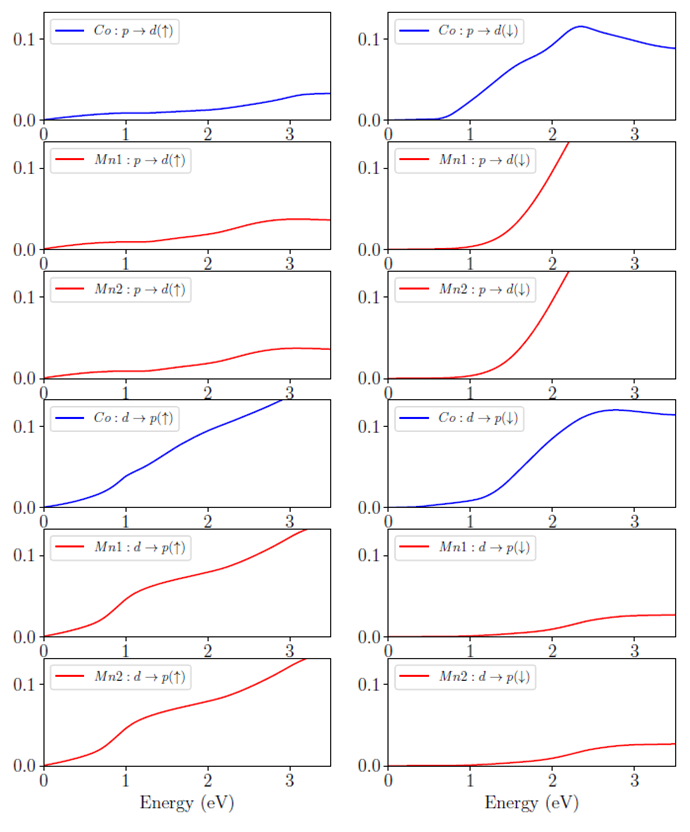
\includegraphics[width=150mm]{figs/TransitionProbB2}
	\end{center}
	\caption{Transition probabilities for the dipole allowed transitions as a function of photon energy in the B2 phase of Co$_2$MnGe. }
	\label{fig: TransitionProbB2}
\end{figure}
The intensity of the transitions from the initial to the final state are provided by the electric dipole transitions and are allowed if a sufficient amount of $d\rightarrow p$ and $p\rightarrow d$ transitions are allowed. Hence, Figs. \ref{fig: Heus4}C and \ref{fig: elementOrbitalDOS} suggests that p-states of Mn and Co that hybridize with d-states are very important in order to enable sufficiently many transitions (illustrated by the red wiggly line in Fig. \ref{fig: Heus4}C of main text). These considerations enable tailoring the optimal condition for spin-moment transfer from one sublattice to another, and could help to find new compounds with even more extreme effects compared to what is reported here in this work.

Next we compute the transition probabilities in the A2 phase. Here both Co and Mn can occupy multiple sites, and probabilities for all site are computed. Note that here the spin polarization at the Fermi level is lost, and as a result transitions in the Mn minority channel become equally probable as those in the majority. The atom-, orbital-, and spin-resolved probabilities are plotted in Fig. \ref{fig: TransitionProbA2}
\begin{figure}[htbp]
	\begin{center}
		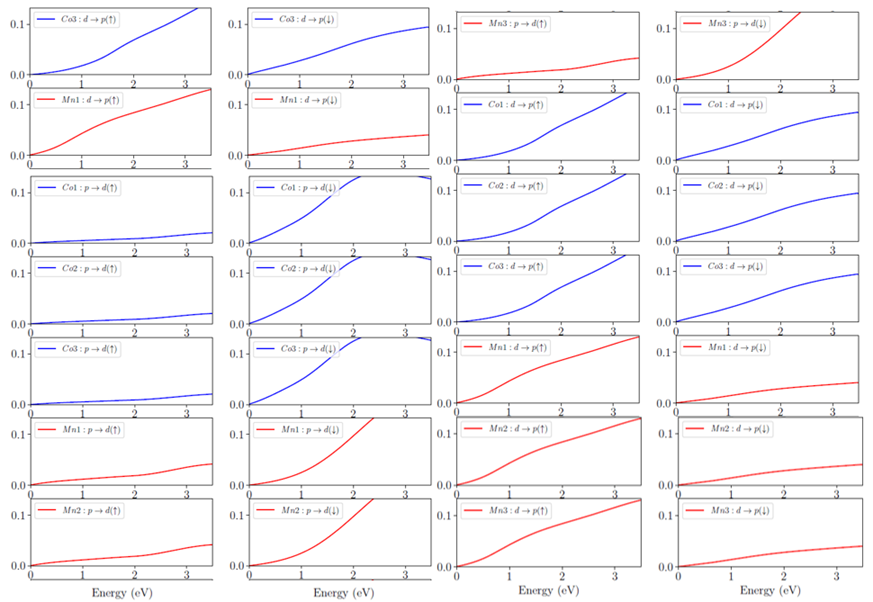
\includegraphics[width=150mm]{figs/TransitionProbA2}
	\end{center}
	\caption{Transition probabilities for the dipole allowed transitions in the A2 phase.}
	\label{fig: TransitionProbA2}
\end{figure}
The total minority and majority band transitions for both Co and Mn are plotted in Fig. \ref{fig: TransitionProbTotalA2}. The probabilities have been normalized by the magnetic moments computed with DFT for both phase (so that there can be direct comparison between A2 and B2 phase probabilities). In the case of Cobalt, transitions from the minority band remain preferred as in the B2 phase. Because of this, we note that the dominant mechanism for spin transfer must come from the blocked spin channel in Mn.
\begin{figure}[htbp]
	\begin{center}
		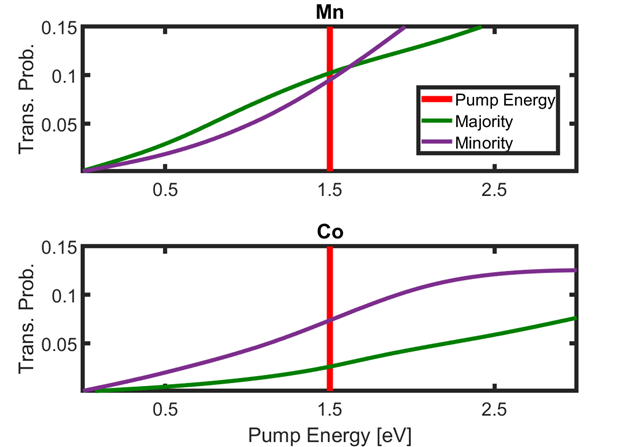
\includegraphics[width=120mm]{figs/TransitionProbTotalA2}
	\end{center}
	\caption{Transition probabilities for the dipole allowed transitions in the A2 phase.}
	\label{fig: TransitionProbTotalA2}
\end{figure}

\section{Results of the calculations of k-conserving transition probabilities for the L21 phase}

Here we compare the simulated transition probabilities, calculated using Eq.\ref{eqn:HeuslerS4} and Eq. \ref{eqn:HeuslerS5}. The difference between them is that in the former case only k-conserving transitions are calculated, whereas in the latter case also non k-conserving contributions enter, due to the two independent k-summations of DOSs. In Fig. \ref{fig: kConsComp} we compare the results for the L21 phase obtained with these two approaches.
\begin{figure}[htbp]
	\begin{center}
		\includegraphics[width=120mm]{figs/kConsComp}
	\end{center}
	\caption{Transition probabilities for the dipole allowed transitions in the A2 phase.}
	\label{fig: kConsComp}
\end{figure}
As one can see, the results are quite similar and are practically identical around the energy of interest, which is 1.5 eV. Since Eq.\ref{eqn:HeuslerS5} is easier to implement, we used it for computing the intensities for the A2 and B2 phases. 

\section{Results of atomistic Landau-Lifshitz-Gilbert simulations}

\subsection{Numerical method}
We consider classical atomic magnetic moments {$m_i$ }=$m_i(e_i)$ at site i. The dynamics of{$m_i$ }  is governed by the atomistic Landau-Lifshitz-Gilbert (aLLG) equation \cite{Antropov1996}
\begin{equation}
\frac{\partial m_i}{\partial t} = m \times (-\gamma(B_i+b_i\frac{\alpha}{m}\frac{\delta m_i}{\partial t}))
\end{equation}
Where $\gamma$ is the gyromagnetic ratio and $B_i$=  $\frac{\partial H}{\partial m_i}$ is the effective precession field related to the spin-Hamiltonian, employing a Heisenberg model where
\begin{equation}
H = - \sum_{i,j}J_{i,j}m_i \dot m_j - \mu_B B \sum_i m_i
\end{equation}
Here, the magnetic moments at site i and j are coupled by the exchange parameter $J_{i,j}$. The values of the Heisenberg exchange parameters were obtained from first principles electronic structure theory. In the expression above, B is the external magnetic field. From the fluctuation-dissipation theorem, thermal fluctuations enter by a stochastic field, $b_i$, that fulfills white noise properties, such as $\braket{b_i}$=0 and $\braket{b_i^\mu(t) b_k^\nu (t')}= D\delta_{i,j} \delta_{\mu \nu} \delta(t-t')$, with the fluctuation amplitude D=2$\alpha k_b$ T/$\gamma$ m . The dissipation part enters the equation of motion via a viscous damping part scaled by the Gilbert damping constant $\alpha$. We address in these simulations the demagnetization as a pure thermal effect in which the temperature of the magnetic sub-system is determined by
\begin{equation}
T = T_0 + (T_p - T_0)(1 - e^{-\frac{t}{\tau_1}})+(T_f - T_0)(1 - e^{-\frac{t}{\tau_2}})
\end{equation}
In this expression, $T_0$ is the initial temperature, where $T_p$ is the peak temperature and $T_f$ is the final temperature. Furthermore, $\tau_1$ and $\tau_2$ are the relaxation times. Note that $T_0$, $T_p$, $T_f$, $\tau_1$ and $\tau_2$ are parameters that determine the profile of the temperature of the spin system. For simplicity, we set $T_0$ = $T_f$ = 300 K, since the simulations were done in order to capture experiments performed at room temperature.

We calculate the dynamics of classical magnetic moments in a simulation box of 10 x 10 x 10 (1000) atoms and with 10 replica, using the UppASD software \cite{Skubic2008}. To guaranty numerical stability, we use a step width of dt = 0.1 fs. Element specific properties are obtained by performing chemical specific averages. In order to reduce even further the numerical noise, an averaging in time is performed for a short period of 100 steps. This period is short enough to not violate non-ergodicity of the process.

\begin{figure}[htbp]
	\begin{center}
		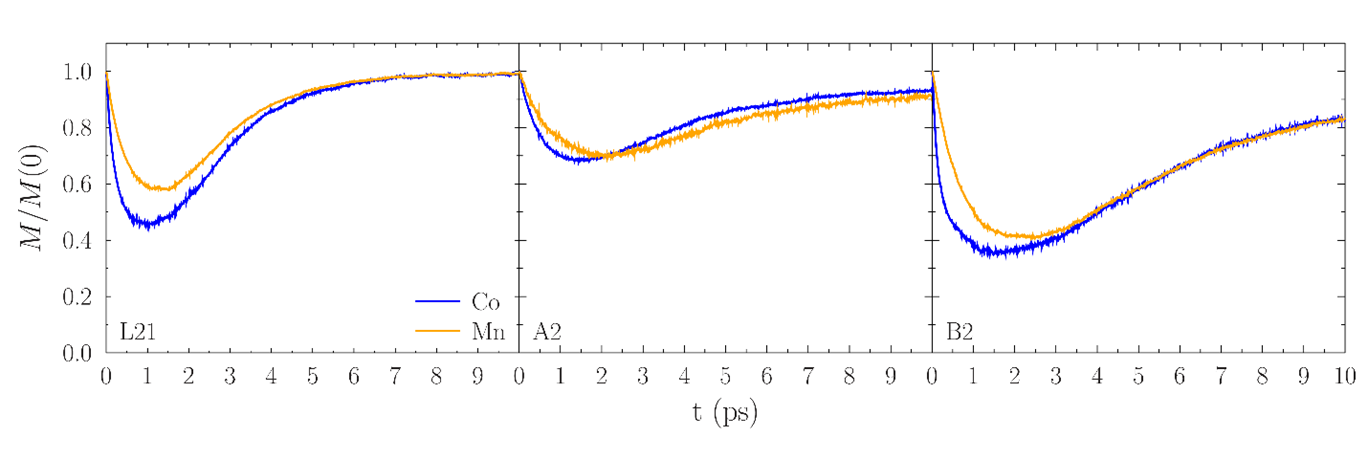
\includegraphics[width=150mm]{figs/LLGResults}
	\end{center}
	\caption{Element resolved demagnetization in Co2MnGe for the L21, A2 and B2 phase. The peak temperature of the simulations is set to 1000 K, whereas the relaxation times of the temperature profile are $\tau_1$= 0.01 ps and $\tau_2$ = 1.5 ps. }
	\label{fig: LLGResults}
\end{figure}

The results of the simulations are shown in the tables following this section. In contrast to the experimental findings, Co demagnetizes faster than Mn. This is because the magnetic moment of the Co atom is smaller than the Mn moment, in all three crystal phases (L21: $\mu_{Co}$ = 0.94 $\mu$B and $\mu$Mn = 3.13 $\mu$B, A2: $\mu_{Co}$ = 1.53 $\mu$B and $\mu_{Mn}$ = 2.54 $\mu$B and B2: $\mu_{Co}$ = 0.93 $\mu$B and $\mu_{Mn}$ = 3.16 $\mu$B), and it can be argued that larger moments have slower dynamics according to the aLLG equation \cite{Mentink2012}. We have furthermore made a fit of the simulated data with a double exponential function (also used in \cite{Malinowski2008});
\begin{equation}
\frac{M(t)}{M(0)}=A_0-A_1e^{-t/\tau_i}-A_2e^{-t/\tau_f}
\end{equation}
The resulting fitting parameters are listed in Fig. \ref{fig: LLGTable1} The relaxation time, $\tau_i$, differs strongly between the different phases and is lowest for the L21 phase. In the A2 and B2 phase, the relaxation time is comparable. The relaxation time for remagnetization, $\tau_f$, is also similar for all three phases. However, both relaxation times depend very strongly on the dissipation term in the equation of motion. In order to apply a complete model, we used type-resolved Gilbert damping parameters, which are listed in Table 2-4 for the particular different phases. The overall results of Fig. \ref{fig: LLGResults} show that the experimental features discussed in the main part of this report, in particular the initial increase of magnetic moment of the Co atoms when the B2 phase demagnetizes, are not reproduced by the aLLG equation. Although some features of the magnetization dynamics seem to be captured by theory at longer time-scales (250 fs and longer), e.g. reaching a minimum at 1.5 – 2 ps with M/M(0) being close to 0.5-0.6, there is a marked difference between theory and experiments for the initial phase of the demagnetization process. This finding is in contrast to earlier calculations for fcc Ni (20) and CoFeB as well as FePt \cite{Hofherr2018}, where theory of this level of approximation reproduces experiments with rather good accuracy. The deviation between experiment and aLLG theory highlights the effects of electronic excitations, that are discussed in Chapter 6 of this thesis.  
